\subsection{Booster Selection - Thomas Satterly}

The booster selection was limited to off-the-shelf boosters, and additional project constraints required that the SFRJ body diameter should not exceed the booster diameter. Basic sizing quickly revealed that the GLD would need as large of a booster as commercially possible, and the Cesaroni Pro 150-40k series was a natural choice. The three variants in the Pro 150-40k are listed in Table \ref{tab:pro150Variants}. 

\begin{table}[H]
    \centering
    \caption{Cesaroni Pro 150-40k Variants}
    \label{tab:pro150Variants}
    \begin{tabular}{l|c|c|c}
          & \textbf{22920O3700-P} & \textbf{37148O4900-P} & \textbf{P40960O8000-P} \\
          \hline
        Burn Time (s) & 8.2 & 7.6 & 5.1 \\
        Total Impulse ($\text{lb}_{f}$*s) & 6726 & 8351 & 9216 \\
        Peak Thrust $\text{lb}_{f}$ & 918 & 1256 & 1935
    \end{tabular}
\end{table}

Each variant was analyzed to determine the maximum payload mass they could accelerate to Mach 2, and the P40960O8000-P proved to be the most capable. The payload was simulated as a dead mass that had a constant drag coefficient of 0.5, which later proved to be too optimistic for a drag estimate, but the overall results still hold. The initial investigation revealed that the P40960O8000-P booster could accelerate approximately 75 pounds to Mach 2, and altering the launch elevation angle would significantly affect the drop altitude. The relationships between payloadd mass, launch elevation angle, and drop conditions are shown in Figure \ref{fig:boostPerformance}.

\begin{figure}[H]
    \centering
    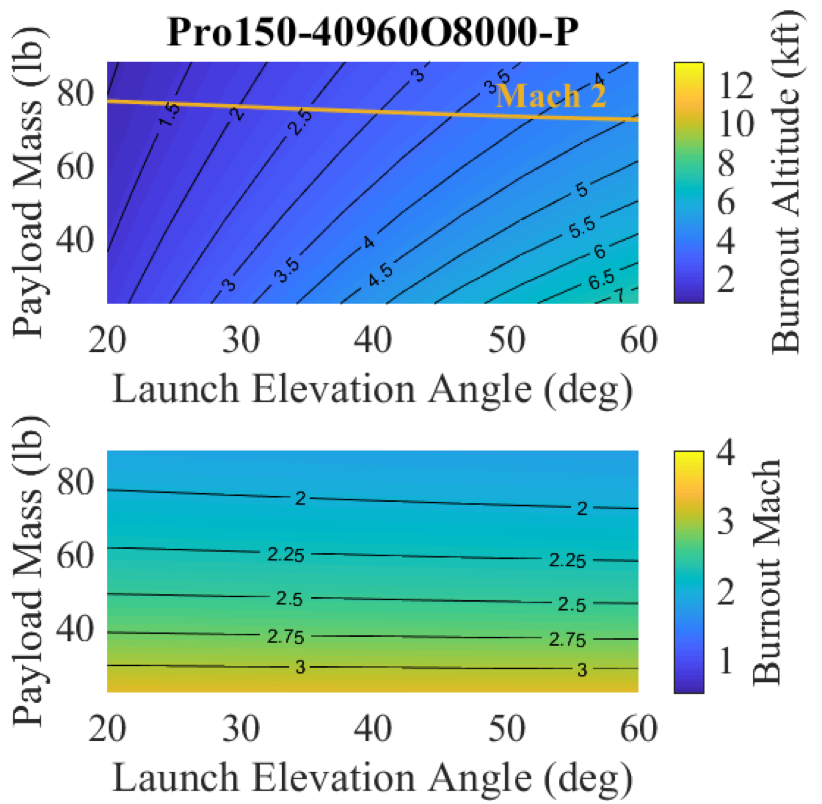
\includegraphics[width=0.7\textwidth]{ParameterSweeps/figures/BoostFig.png}
    \caption{Performance Capability of Cesaroni Pro 150 Booster}
    \label{fig:boostPerformance}
\end{figure}

The launch elevation angle has an immediate and significant effect on the drop condition altitude, but it is also worthwhile to consider the pitch maneuver required to bring the SFRJ to level flight as well as the altitude gain during the pitchover maneuver. 